%# -*- coding: utf-8-unix -*-
%%==================================================
%% chapter01.tex for SJTU Master Thesis
%%==================================================

%\bibliographystyle{sjtu2}%[此处用于每章都生产参考文献]

\chapter{绪论}
\label{chap:intro}
\section{语言模型及其研究背景}
随着计算机运行速度的提升和机器学习领域的发展,机器学习已经成为当今大的研究趋势。
智能语音可以让计算机听懂甚至理解人类的语言,因此成为了智能交互中很重要的一部分,语言模型的作用功不可没。
同时,大规模语料库的出现和现代计算机计算能力的提升,为自然语言统计处理方法的实现提供了可能,统计方法的成功使用推动了语言模型的发展。
语言模型作为衡量一句话的流畅及合理程度的模型,语言模型在语音识别和自然语言处理任务中都得到了广泛的应用。
在自然语言处理任务中,语言模型不仅可以用来衡量语句的符合语言规律及通顺程度,更可以和众多别的自然语言处理任务相辅相成,相互促进。
在语音识别任务中,语言模型和声学模型合作完成,通过解码过程将音频信息转化为最为合理的文字。
本论文着重介绍语言模型在语音识别任务中的研究和优化。



自古以来,语音都是人类最重要的交流方式之一。
自电话发明以来,学者们致力于机器的语音的研究工作。
19世纪晚期,在语音工作的种种问题中,自动语音识别(Automatic Speech Recognition,ASR)成为最具挑战性和吸引力的任务之一,它是通过先记录语音波形并通过一系列算法自动转换为文本。
然而,对ASR的研究在20世纪初却进展缓慢,甚至1969年,贝尔实验室的约翰·皮尔斯还曾声称自动语音识别在几十年内不会成为现实。


不过,在十九世纪70年代,语音识别领域有了巨大的突破。
各类方法在语音识别领域崭露头角,其中就包括语言模型。
在接下来的几十年里,随着机器学习方法的提出,和深度学习的证实与应用,神经网络被用于语音识别领域。
基于神经网络的各种语言模型训练方法也逐步进入研究者的视角。
在此基础上,各种结构化神经网络的语言模型相关研究再一次推动了语言模型的性能和应用空间。


语音识别系统的目的是能通过给定的语言波形而产生一个单词序列(或者可能是适用于普通话之类语言的汉字序列)。


ASR系统的基本结构如图\ref{fig:asr}所示\cite{mohamed2012acoustic}。



\begin{figure}[!htbp]
  \centering
  \begin{minipage}[b]{0.6\textwidth}
    \captionstyle{\centering}
    \centering
    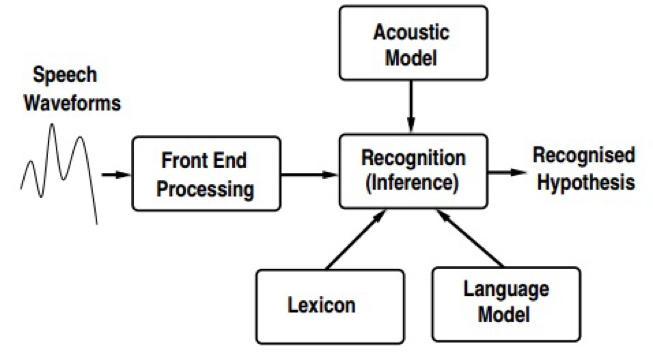
\includegraphics[width=12cm]{intro/ASR.png}
    \bicaption[fig:asr]{自动语音识别系统}{ASR structure}{Fig}{自动语音识别系统的结构}
  \end{minipage}     
\end{figure}

语音识别的第一阶段是压缩语音信号(逐帧)为声学特征向量的流, 称为观测值。

提取的观测向量被设计成包含足够的信息以及足够紧凑来执行有效的语音识别。
这一过程被称为前端处理或特征提取。
/
从观测特征向量说开来,ASR系统可分为三个主要部分:词汇,语言模型和声学模型。

词汇或者称为词典,用于映射出在声学模型中的子字单元到词汇与语言模型中的实际单词。
语言模型代表了已说出句子的当地句法和语义信息。
它对每个单词序列都分配了个可能性。
声学模型,通常是语音研究者们最感兴趣的,映射了语音观测值到子字单元。
 GMM-HMM框架一直是ASR框架的最先进技术,直到最近深度神经网络(DNN)被引入到ASR系统中。
计划中的深度神经网络HMM(DNN-HMM)相比于最先进的GMM-HMM来说在两种任务上都取得了显著进步,音素识别\cite{mohamed2012acoustic}和大词汇连续语音识别(LVCSR)\cite{dahl2012context}任务。
它使用一个深度神经网络(DNN)来计算聚类后状态并将其转换为可用于HMM的状态和条件似然概率。


深度神经网络(DNN)比起浅层的神经网络有更强大的模拟/建模能力。
但是, 它也更有可能因为正常初始化策略和反向传播(BP)优化而陷入局部的最优。
RBM(受限玻耳兹曼机)的预训练\cite{mohamed2012acoustic}或区别预训练\cite{bengio2007greedy}被提出来用作初始化权重矩阵到一个更好的起点,这使BP微调过程更容易,而且收敛更快速。
最近,文献\cite{mohamed2010investigation}\cite{vesely2013sequence}介绍了更先进的训练标准,它们已被应用于得到更精确的模型。
除了混合框架,DNN也可以用于获得更完善的瓶颈特征\cite{yu2011improved},以训练GMM-HMM系统并已经实现了与DNN相匹配的性能。


随着自动化语音识别的不断优化和发展,在识别中扮演重要角色的语言模型的研究同样得到迅速发展。
从传统的统计学语言模型N-gram到神经网络语言模型,从普通的深度神经网络语言模型到有历史记忆功能的循环神经网络,再到更优秀但是更复杂的长短时间变化神经网络,甚至是各种对模型结构上的优化,一步步使语言模型研究更加深入,从而大幅度提升语言模型的性能。



\section{语言模型的相关研究}
在20世纪90年代,最初的语言模型N-gram语言模型开始被提出。
N-gram语言模型原理简单,仅需要掌握简单的概率论基础知识和极大似然概率就能实现,而且速度很快,对于当时的计算机硬件条件来说适用性很高,很快就被广泛接受和应用开来。
这样一来,很多缺点和不足也就暴露出来,比如当训练数据不足的情况下很容易出现很多单词的预测概率为0,于是就有很多学者提出各种平滑算法来解决语料稀疏的问题。
比如基于二项后验分布的后退(back-off)平滑方法\cite{kawabata1996back},
基于普通计数的平滑方法\cite{moore2009improved}
和Kneser-Ney平滑\cite{pickhardt2014generalized}等。
其中Kneser-Ney平滑算法是目前比较标准的,而且是非常先进的平滑算法。

除了这些平滑算法,在N-gram的训练形式和语料的预处理方面专家们也是下足了功夫,
例如基于缓存的(Cache-based N-gram模型用缓存记录历史信息\cite{kuhn1990cache},
基于类别的(Class-based)N-gram模型将单词进行分类处理\cite{brown1992class}
以及基于话题的(Topic-based)N-gram模型在训练单词的时候为其配备话题附加信息以达到更好的训练等\cite{gildea1999topic}。

随着21世纪深度学习方法被证实可用,神经网络算法开始被用于自动语音识别和语言模型的学习当中。
开始的DNN算法由于无法记录较长的历史信息而不适用于语言模型,因为语言是具有前后文连贯性的。
接着随着RNN语言模型的提出,发现具有递归结构能够记录历史信息的循环神经网络(Recurent Neural Network,RNN)网络非常适用于语言模型。

RNN由于递归结构的存在使得语言的历史信息能够被记住,十分符合语言学的规律,使得语言模型的性能从统计模型N-gram有了很大的提升。
同时RNN模型的训练方式也从以前普通DNN的反向传播算法(BP)变化成了基于时间的反向传播算法(BPTT),这个算法将会在第二章进行详细介绍。
同样的,学者将优化N-gram语言模型的思想扩展到语言模型上,提出一系列优化RNN语言模型的算法。
例如Class based RNNLM被提出,它的思想同N-gram一样,对训练单词进行分类训练,能够有效的提高训练速度,并且对于丰富多彩的语言来说,那些出现概率偏小的词汇在预测中容易导致概率为0的问题得到了平滑。
优化深度神经网络(DNN)的各种训练算法同样适用于RNN语言模型的训练,从开始的一个词一个词的训练的随机梯度下降,到多个词同步训练的批量梯度下降,以及训练中加入块的机制,都大幅度提升了RNN模型的训练速度,同时也一定程度提升了语言模型的性能。
从语言模型训练速度的方向考虑,以前的语言模型不能同声学模型一样进行minibatch训练(nimibatch即是把训练数据分批输入到神经网络中进行学习),因为语言模型的识别往往和前后文以及历史信息关系密切,然而去年有学者提出可以换种方式考虑minibatch,同时读入很多句子,在不同的没有关联的句子中选取不同的单词进行minibatch输出,则不会影响学习相关性的情况下还能对速度有所提升。
另外多核并行学习,利用GPU和Intel函数库进行训练等方法逐渐被用于语言模型训练上。

然而RNN语言模型依然有一个普遍存在的问题——梯度消失。
即当语句过长时,距离现在较长的历史会随着一步步的递归使得历史影响消失,这种情况使得RNN虽然理论上能用到的历史信息是全部历史,但是真正产生作用的历史信息依然非常有限。
针对这个问题,
有人提出加入长短时间记忆(LSTM)的神经网络语言模型来学习那较长的句子。面对这些些有很长一段时间信息滞后并且滞后时间的长短未知的句子,它通过分割记忆块的形式控制误差的传递时机,训练得到语言模型的性能相比传统RNNLM具有一定提升。
好在无论是训练方法的提升(小批量随机梯度下降),还是计算方法的提升(多线程GPU并行)以及硬件计算能力的提升为训练具有相对于RNN来说几倍参数量的LSTM模型提供了可能性。

在上述技术基础上,针对基础语言模型进行的各种创新结构的研究也在紧锣密鼓的进行。
多视角(Multi-view)语言模型是将多种特征向量加入到语言模型中辅助训练更好的语言模型的结构,
比如加入前后文相关信息的RNN语言模型于近年被Mikolov提出,它在训练当前单词的时候加入前后文块,并为词性加入话题信息,结合话题模型一起进行训练,形成一个受话题制约的RNNLM,可以有效避免数据在不同类型的数据子集上训练话题模型导致的数据分裂。
多任务(Multi-task)学习同样受到了很大的关注,其主要思想是在训练语言模型时加入其它的任务混合训练,共用一定数量的隐藏层或参数矩阵,达到相互促进相互制约的作用。
联合学习(Joint train)作为多视角和多任务模型的结合,也是最复杂的一个。
不仅像多视角模型一样拥有多维视角特征,也像多任务学习一样多种不同任务共同学习以达到相互促进和泛化的作用。
往往多任务的输出会以各种经过尝试的较好方式作为额外视角加入到下个时间点的训练中。

上述提到的各种语言模型的结构化尝试也是本文的工作重点,额外的丰富的信息和合理的结构往往能使语言模型发挥更好的效果。







	
\section{本文的研究内容及贡献}

本课题主要研究面向ASR的结构化的语言模型,以提升语言模型的性能。
首先,本文调研所有现有的结构化语言模型的研究现状和它们的优缺点,以得到研究的突破点:大多数结构化模型的研究都仅仅提升了混淆度,而没有提升ASR重打分任务中的指标。
接着本文分析造成这个现象的原因:用不应该使用的含有后文信息的标注预测后文信息使得混淆度有巨大提升,但是这种提升是用到了作弊的后文信息,
而在语音识别的N-best重打分任务中,后文的信息不一定正确因此没有提升。
于是有了本文主要工作的研究动机:将单向信息抽象出来,进行Multi-view语言模型的训练,然后在N-best重打分实验中验证结果。


由于词层面的Multi-view必须使用此层面的信息。
为此我们优先调研有哪些词层面的信息,且哪些可以被用在我们的研究中。
最后得到了三种辅助特征:词性标注(POS),命名实体识别(NER),语法块标注(Chunking)。
其中有些可以直接通过现有工具获得标注,有些需要自己根据论文实现标注工具。

接下来是为结构化语言模型的研究作为辅助任务但仍十分钟要且有一定研究成果的任务:面向结构化语言模型的学习率自适应算法。
由于结构化的模型中,不同的结构会有不同的特性,且训练步调也不一定会一致,因此使用同一种学习旅会影响模型的学习效果。
我们在已有的$beta$稳定算子学习率自适应算法中,将其移植到LSTM语言模型中,保持了原有的效果,即使得模型对初始学习率不敏感,能自动调整模型在训练过程中的学习幅度,
从而使得无论是Multi-task还是Multi-view或者是Joint-train模型都能根据没一部分的特性有“个性”地进行学习。
在此基础上,对$beta$进行L2正则化优化,使其能一定程度上($1\%$)提升模型性能。
研究完整且颇有成效,最后我们也是将这个研究成果运用到本文的结构化语言模型的研究中去,最后使得研究更为系统和有说服力。

在本文的主要研究内容中,在上述辅助特征的选取和学习率自适应的基础上。
本文提出面向ASR的单向辅助信息的Multi-view语言模型,模型是一个整体,但是分成标注LSTM和Multi-viewLSTM语言模型两部分。
意在将不含后文信息更准确的辅助特征加入到语言模型中一起训练。
并且含有多种连接方式和多种训练方式。最后通过实验验证哪种方式更好,以及模型是否有效果。

实验部分首先选取合适的数据集,本文选取了中文和英文的数据集以试图得到更为普遍的结果。
在英文数据集上,也选取了较大的和较小的两种,其中中文和英文大数据集是能进行N-best重打分实验的。
除此之外还要将数据集预处理,分别通过对应的算法得到数据对应的词性、话题和场景等不同的信息,并进行标注得到新的数据集。
然后,以词为单位对带标记的数据进行解析,得到其词向量和对应信息的特征向量。
最后将这些向量一同作为标注模型进行训练。
模型的基线也是非常全面,除了统计学N-gram模型之外,还有普通的LSTM语言模型,和基础的Multi-view、Multi-task、Joint-train语言模型三种,来测试我们的模型。
并在实验部分给出了完整的实验数据和分析比较。

最后证实本模型在ASR任务的WER和SER指标上分别有平均$4\%$和$2\%$的提升,比较显著。
成功提升了语言模型在语音识别中的应用性能。





\section{论文结构}
本论文剩下的部分是这样组织内容的:
第二章主要介绍什么是语言模型,语言模型的作用,以及各种语言模型。。
首先介绍最基本的,出现最早也是应用范围最广的N-gram语言模型,它是非神经网络语言模型,本文着重从它的定义和结构,以及数学原理等方面进行分析,然后简单介绍它的优化和变形,在第五章N-gram开源工具srilm将会作为实验对比工具出现。
然后引入当前应用最广的神经网络语言模型,不仅从概念上介绍神经网络的定义,更是从数学原理、模型结构及训练的角度阐述神经网络语言模型。
在此基础上由浅入深地介绍从基础的循环神经网络语言模型(RNNLM)到效果更好但更为复杂的长短时间变化(LSTM)RNNLM的各种细节。
毫无疑问,这部分是本论文和本人研究生阶段的研究工作的基石,


第三章主要介绍面向结构化语言模型的$beta$稳定算子自适应算法。
先解释了历史研究和研究动机。
然后在历史研究的基础上介绍了我们将其加入到LSTM语言模型中的方法和原理,并详述其数学原理。
最后介绍了加入L2范数的优化。


第四章是本文最重要的章节,也是本文工作内容和贡献所在——深入探讨结构化语言模型的研究。
前半章是各种结构化语言模型已有工作的调研和实验的复现。
主要根据结构的特征分为Multi-task、Multi-view和Joint train三种不同的模型结构。
分别详细介绍这三种结构的特征、表现和各自的优缺点。
后半章详细介绍本文的三个主要工作:内容及创新点,以及研究的步骤、技术细节和进展。
首先介绍本文在研究中主要用到的三种辅助维度:词性(POS)、命名实体(NER)、语义块标注(Chunk),以及他们对语言模型的训练有何积极作用,然后分别提出各自的特征向量提取方法。
紧接着本文提出单向自信息Multi-view和Joint train模型的结构,包括模型结构的动机,不同的训练方法的尝试以及本模型的创新点及优势。
另外本文还介绍了Teacher-student的相关研究和细节。




第五章是实验与分析部分,
首先引入实验的基础知识,同时介绍实验的平台、数据集等一系列相关内容。
然后介绍实验的设计和流程,本文将从上述三种基础结构和本文的两种创新结构出发,进行全面的实验和对比。
最对所有的实验数据进行展示、对比、分析,得出结论并进行总结。



